%!TEX root = thesis.tex
\chapter{2-D Imaginary Time Evolving Block Decimation}
\label{chapter:2ditebd}

In this chapter we introduce some different ways to implement two-dimensional imaginary time-evolving block decimation and apply them in calculation of ground state of Heisenberg and transverse Ising model on two-dimensional square lattice. In section \ref{ite} and \ref{itebd}, we briefly review the idea of imaginary time evolution (iTEBD),[\ref{vidal}] and explain how to extend it to two-dimensional [\ref{X,zhon}]. Second, we briefly review another method to make 2D-iTEBD more stable[\ref{1.1}]. In the last section \ref{2dopt}, we record various particulars which are helpful optimizing algorithms.

\section{Imaginary Time Evolution}
\label{ite}
Theoretically, if having the imaginary time evolution operator $e^{-\tau H}$, we could project any random states to the ground state, as long as the wave-function can be written as,
\begin{align}
	\label{mapgroud}
	\Ket{\psi_0} = \frac{e^{\tau H} \Ket{\Psi}}{\parallel e^{\tau H} \Ket{\Psi}\parallel}
\end{align}
but according to the eq.\ref{mapgroud}, we may found that the number of coefficients in an origin evolution operator $e^{-\tau H}$ is proportional to $2^N \times 2^N$. On the other words, it is impossible to update entire system directly. In order to restricting the rapid dimensional growth, we apply \textit{Suzuki Trotter decomposition}[\ref{1.1}][\ref{1.1}] to approximate. The main idea of \textit{Suzuki Trotter} is decomposing the whole system to lots of units cell and using some smaller operations to update the wave-function.
\begin{align}
	\label{STd}
	e^{\delta A + B} = e^{\delta A}e^{\delta B} + O(\delta^2)
\end{align}
eq.\ref{STd} means the first-order Suzuki Trotter  decomposition, and A and B are non-commutative with each other.

Now that the dimension of the evolution operator is reduced to a n-site operator and in chapter \ref{chapter:properties}, we have shown that a many-body system can map to a MPS or PEPS structure, so we can draw the process of updating a ground state like Fig.\ref{fig312},

\begin{figure}[ht]
	\centering
	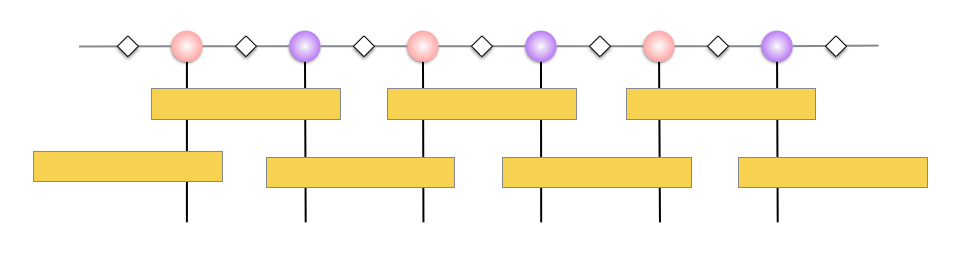
\includegraphics[width=0.75\textwidth]{figures/fig312.png}
	\caption[The picture of the main idea of itebd.]{The red and blue tensor denotes on \textit{odd} and \textit{even} sites. The yellow one are time evolution operators $e^{-\tau H_{k,k+1}}$, $e^{-\tau H_{k+1,k}}$}
	\label{fig312}
\end{figure}

On the other work, contract the tensors in Fig.\ref{fig312} repeatedly until the ground state energy to the minimum. The remained tensor is considered as the ground state of the system. So the next question: How can we contract them and preserve the structure like Fig{\ref{fig311}}? This answer is iTEBD.

\begin{figure}[ht]
	\centering
	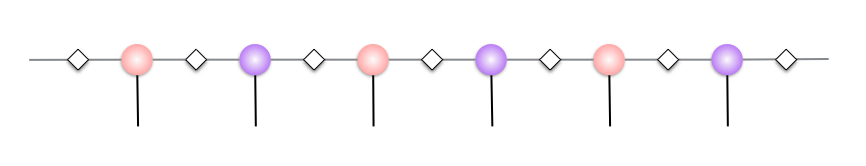
\includegraphics[width=0.75\textwidth]{figures/fig311.png}
	\caption[The picture of matrix product states]{The simple form of a matrix product state.}
	\label{fig311}
\end{figure}

\section{Simple Infinite Imaginary-Time Evolving Block Decimation for 2-D system}
In this section, we apply the TN diagrams to introduce the methods of implementation of algorithm. If you are interested in the mathematical formula of them, please read the references[\ref{22}][\ref{dd}][\ref{eaef}], witch include more details of theoretical discussion.

\label{itebd}
\subsection{Simple Infinite Imaginary Time Evolving Block Decimation for 1-D system}

The algorithm start from 2 random states and 2 random diagonal matrices which are considered as entanglement between particles. In the TN diagrams, Fig.\ref{fig313}, the states and entanglement between neighbor sites are represented by the nodes and bonds with different colors.

\label{1ditebd}
\begin{figure}[ht]
	\centering
	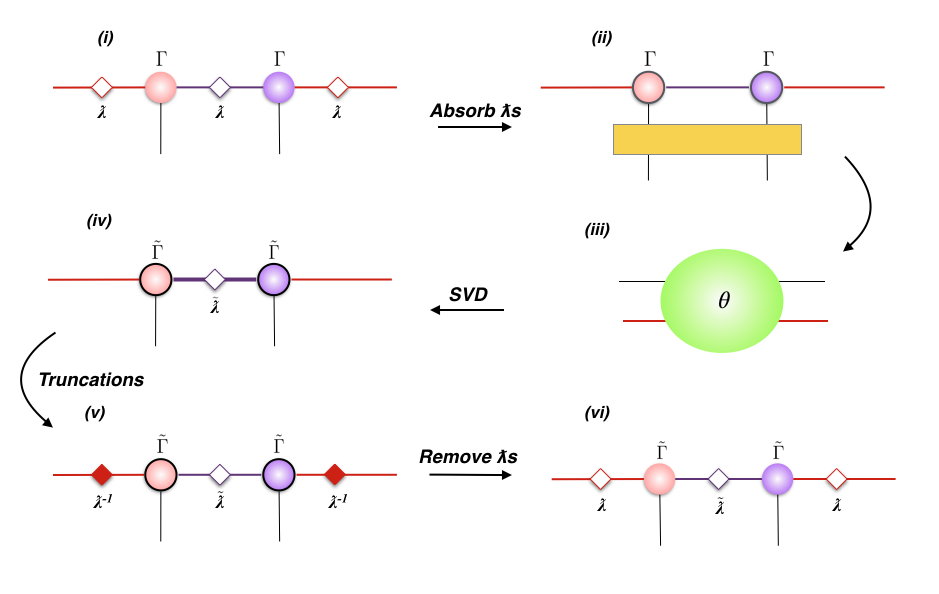
\includegraphics[width=0.75\textwidth]{figures/fig313.png}
	\caption[The tensor network diagrams for the 1-D iTEBD]{ (i)Absorb all $\lambda$ to $\gamma$. (ii) Contract an evolution operator $e^{-\delta H}$ for evolving the system. (iii) Decompose the tensor $\theta$ by SVD. (iv) Truncate and Update the states and $\lambda$ on the green bond.(v) Remove $
		\lambda$ for obtaining the states. (iv) After updating the states and $\lambda$ on the purple bond, apply the way to update the red bond and repeat all the steps until the ground state convergence.}
	\label{fig313}
\end{figure}

The processes shown in Fig.\ref{fig313} is a standard strategy for implementation of iTEBD and also called \textit{Simple Update}. 

In one dimensional system, the performance of Simple Update is pretty well, because 1-D systems obey the canonical form and have less influences of environment. However, in 2-D systems, due to the area law, we need consider the environment more restrictively when measuring the local observable. Moreover, the computational consumption is another serious problem, owing to the growth of a state's dimension which is proportional to $dD^4$.

In order to solving that obstacles, optimizations of 2-D algorithms  became an important part in condense matter physics. This chapter we focus on obtaining good enough projected entangled pair states from 2-D iTEBD and the strategies of improving measurement would be shown in following chapters.

\subsection{Description and Pseudocode of iTEBD for 2-D system}
\label{2ditebd}

Now that we stated to extend it to a two dimensional system. In chapter.\ref{chapter:properties}, we have known that a two dimensional many-body system is able to be represented by PEPS. Due to impossibly drawing an network of infinite sites, the structure of infinite PEPS (iPEPS) is decided by the geometry of the lattice and the unit cell we chosen. In usual, the size of unit cell depend on the n-site evolution operator. For instance, if the target is updating iPEPS of a square lattice with 2-site operator, the tensor diagram would be drawn as Fig.\ref{fig314}.

\begin{figure}[ht]
	\centering
	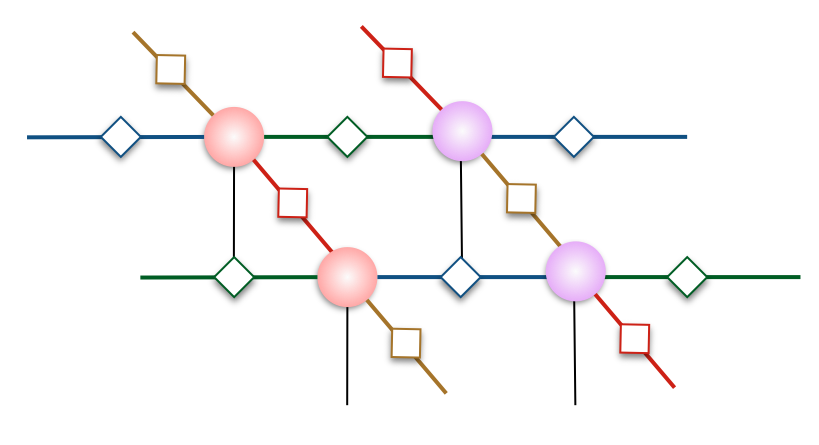
\includegraphics[width=0.6\textwidth]{figures/fig314.png}
	\caption[The tensor diagrams of 2-D lattice]{Four sites unit cell in iPEPS.}
	\label{fig314}
\end{figure}

After setting the form of iPEPS, we start to deal the question of updating states. The most intuitive scheme is to apply the scheme of \textit{Simple Update} which is shown in Fig.\ref{fig315} . The steps is similar to the iTEBD on 1-D systems. However, there are some differences. First, the projected entangled pair states is a rank-5 tensor. Second, there are more entangled should be considered, due to having more neighbor sites.

The more theoretical description is written in [\ref{}][\ref{}]. Here, we explain the methods with TNs and some simple pseudocode.

	\begin{figure}[ht]
	\centering
	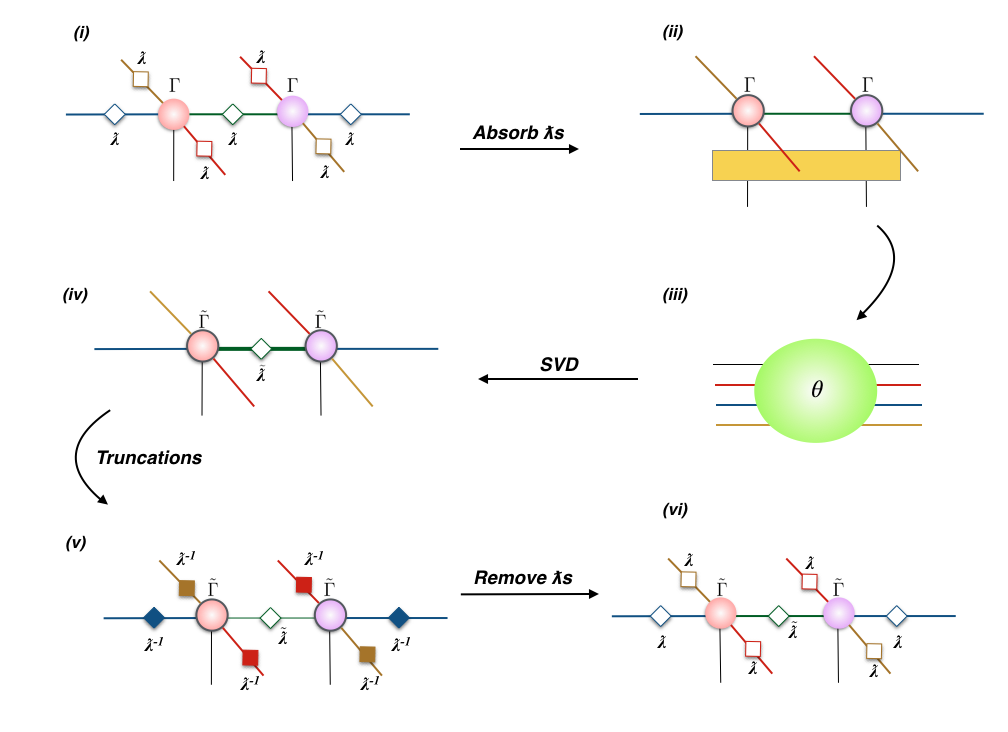
\includegraphics[width=0.75\textwidth]{figures/fig315.png}
	\caption[The tensor network diagrams for the 2-D iTEBD]{}
	\label{fig315}
\end{figure}

\begin{algorithm}
	\caption{My algorithm}\label{euclid}
	\begin{algorithmic}[1]
		\Procedure{MyProcedure}{}
		\State $\textit{stringlen} \gets \text{length of }\textit{string}$
		\State $i \gets \textit{patlen}$
		\BState \emph{top}:
		\If {$i > \textit{stringlen}$} \Return false
		\EndIf
		\State $j \gets \textit{patlen}$
		\BState \emph{loop}:
		\If {$\textit{string}(i) = \textit{path}(j)$}
		\State $j \gets j-1$.
		\State $i \gets i-1$.
		\State \textbf{goto} \emph{loop}.
		\State \textbf{close};
		\EndIf
		\State $i \gets i+\max(\textit{delta}_1(\textit{string}(i)),\textit{delta}_2(j))$.
		\State \textbf{goto} \emph{top}.
		\EndProcedure
	\end{algorithmic}
\end{algorithm}

\section{Ameliorate two-dimensional iTEBD}
\label{2dhastin}

	\begin{figure}[ht]
	\centering
	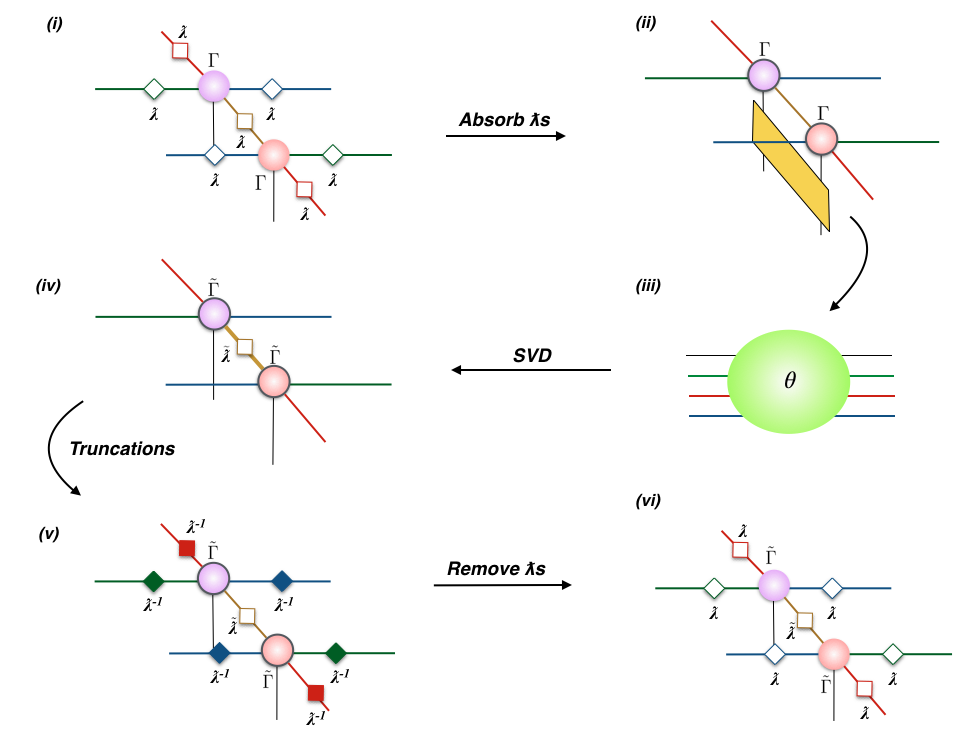
\includegraphics[width=0.75\textwidth]{figures/fig316.png}
	\caption[The tensor network diagrams for the 2-D iTEBD which is ameliorated by Hestins]{}
	\label{fig316}
	\end{figure}

\section{Optimizations}
\label{2dopt}

\subsection{QR decomposition}
\label{2doptQR}
	\begin{figure}[ht]
	\centering
	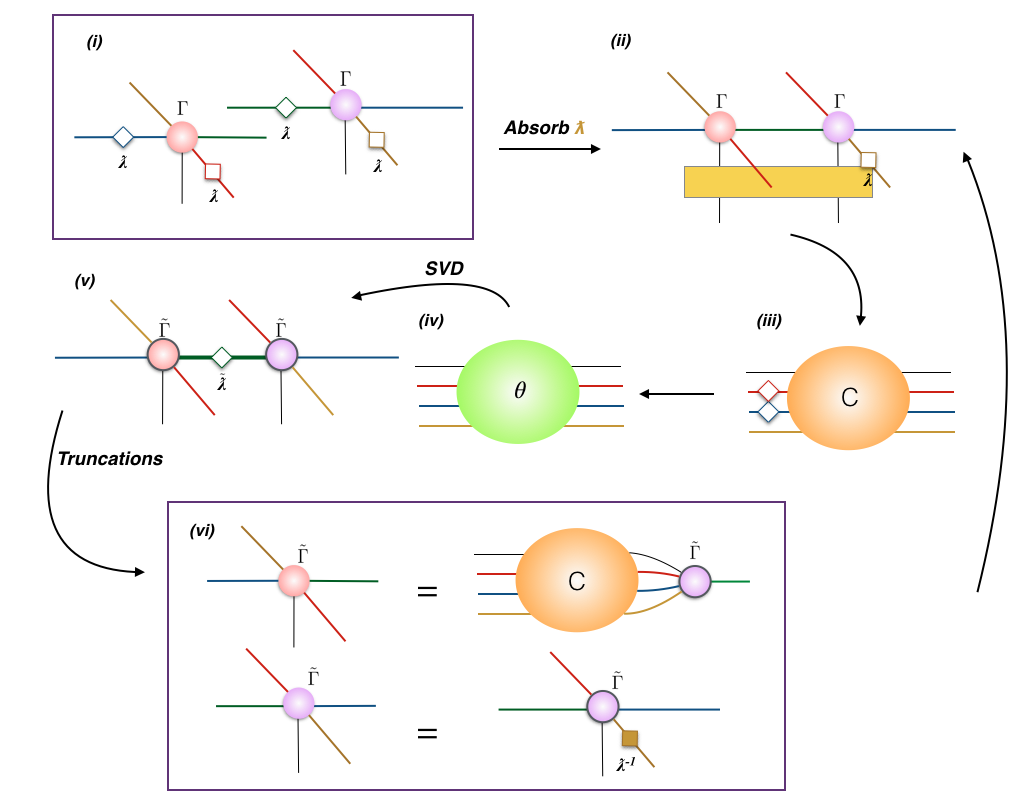
\includegraphics[width=0.75\textwidth]{figures/fig317.png}
	\caption[The tensor network diagrams for the 2-D iTEBD with QR decomposition]{}
	\label{fig317}
	\end{figure}

	\begin{figure}[ht]
	\centering
	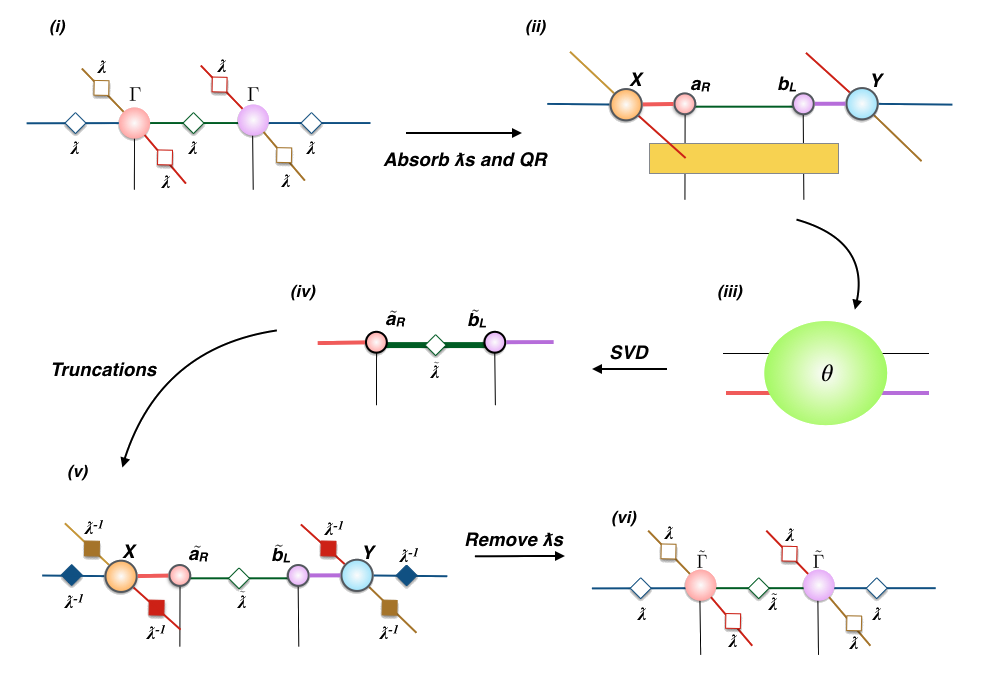
\includegraphics[width=0.75\textwidth]{figures/fig318.png}
	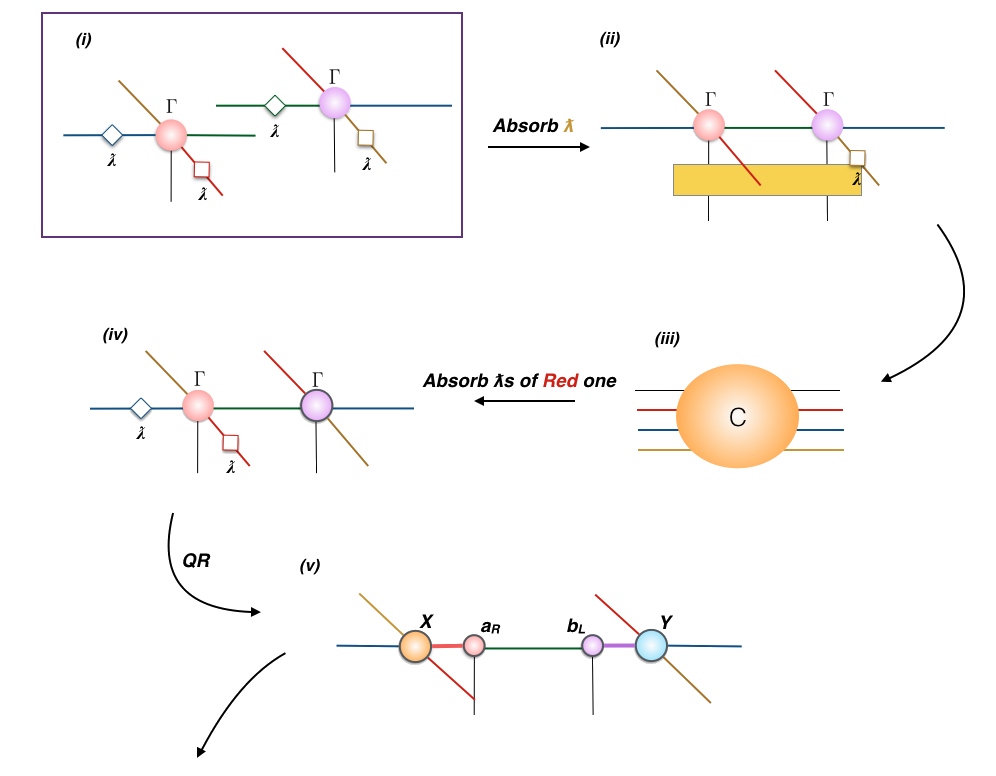
\includegraphics[width=0.75\textwidth]{figures/fig319.png}
	\caption[The tensor network diagrams for the ameliorated 2-D iTEBD with QR decompositiont]{The tensor network diagrams for the ameliorated 2-D iTEBD. More explicitly discussion are in	this paragraph}
	\label{fig318}
	\end{figure}

\subsection{Initialization}
\label{2doptInit}

